\documentclass[border=4pt]{standalone}
\usepackage[T1]{fontenc}
\usepackage{mathptmx}
\usepackage{amsmath,amssymb}
\usepackage{xcolor}
\usepackage{tikz}
\usetikzlibrary{positioning,arrows.meta,fit,calc,shapes.geometric,backgrounds}
\definecolor{bmain}{HTML}{0F4D92}
\definecolor{bsec}{HTML}{3775BA}
\definecolor{blight}{HTML}{DCE8F5}
\definecolor{gfill}{HTML}{DDF3DE}
\definecolor{gline}{HTML}{5BAF5B}
\definecolor{rfill}{HTML}{F6CFCB}
\definecolor{rline}{HTML}{B64342}
\definecolor{nfill}{HTML}{EFEFEF}
\definecolor{nline}{HTML}{767676}
\definecolor{ink}{HTML}{272727}
\tikzset{
  >={Stealth[length=4pt]},
  box/.style={draw=nline, fill=nfill, rounded corners=2pt, align=center, inner sep=4pt, line width=0.6pt, text=ink},
  ours/.style={draw=bmain, fill=blight, rounded corners=2pt, align=center, inner sep=4pt, line width=0.9pt, text=ink},
  data/.style={draw=gline, fill=gfill, rounded corners=2pt, align=center, inner sep=4pt, line width=0.6pt, text=ink},
  warn/.style={draw=rline, fill=rfill, rounded corners=2pt, align=center, inner sep=4pt, line width=0.6pt, text=ink},
  arr/.style={->, line width=0.8pt, draw=ink},
  lab/.style={font=\footnotesize\itshape, text=nline, align=center},
}
\newcommand{\ffpp}{FF\texttt{++}}

\begin{document}
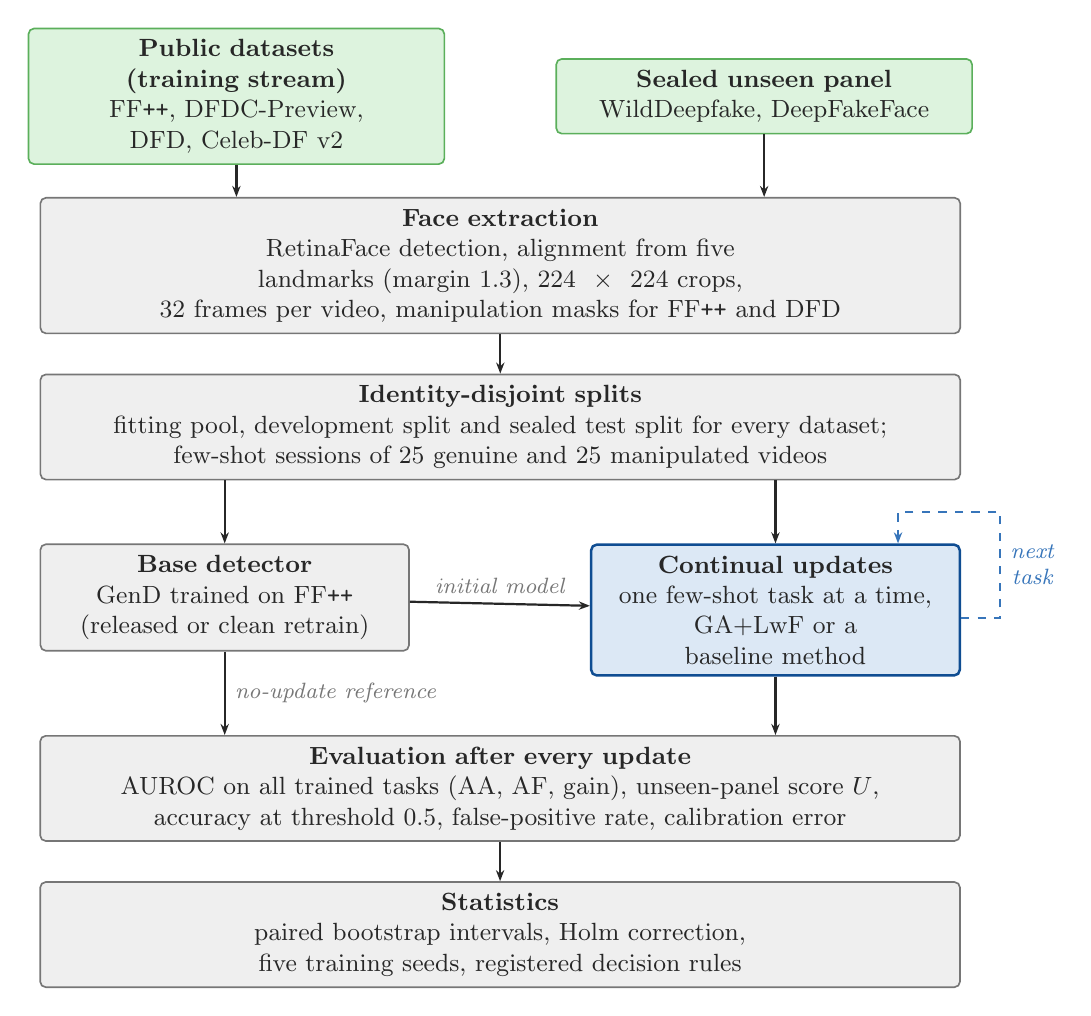
\begin{tikzpicture}[font=\small, node distance=5mm and 6mm]
\tikzset{wide/.style={text width=11.4cm}}
\node[data, text width=5.0cm] (raw) {\textbf{Public datasets (training stream)}\\ \ffpp{}, DFDC-Preview, DFD, Celeb-DF v2};
\node[data, text width=5.0cm, right=14mm of raw] (sealed) {\textbf{Sealed unseen panel}\\ WildDeepfake, DeepFakeFace};
\node[box, wide, below=6mm of $(raw.south)!0.5!(sealed.south)$] (pre) {\textbf{Face extraction}\\ RetinaFace detection, alignment from five landmarks (margin 1.3), $224\times224$ crops,\\ 32 frames per video, manipulation masks for \ffpp{} and DFD};
\node[box, wide, below=of pre] (split) {\textbf{Identity-disjoint splits}\\ fitting pool, development split and sealed test split for every dataset;\\ few-shot sessions of 25 genuine and 25 manipulated videos};
\node[box, text width=4.4cm, below=8mm of split.south west, anchor=north west] (base) {\textbf{Base detector}\\ GenD trained on \ffpp{}\\ (released or clean retrain)};
\node[ours, text width=4.4cm, below=8mm of split.south east, anchor=north east] (upd) {\textbf{Continual updates}\\ one few-shot task at a time,\\ GA+LwF or a baseline method};
\node[box, wide, below=9mm of $(base.south)!0.5!(upd.south)$] (eval) {\textbf{Evaluation after every update}\\ AUROC on all trained tasks (AA, AF, gain), unseen-panel score $U$,\\ accuracy at threshold 0.5, false-positive rate, calibration error};
\node[box, wide, below=of eval] (stat) {\textbf{Statistics}\\ paired bootstrap intervals, Holm correction, five training seeds, registered decision rules};
\draw[arr] (raw.south) -- (raw.south |- pre.north);
\draw[arr] (sealed.south) -- (sealed.south |- pre.north);
\draw[arr] (pre) -- (split);
\draw[arr] (split.south -| base.north) -- (base.north);
\draw[arr] (split.south -| upd.north) -- (upd.north);
\draw[arr] (base) -- node[above, lab]{initial model} (upd);
\draw[arr] (upd.south) -- (upd.south |- eval.north);
\draw[arr] (base.south) -- node[right, lab]{no-update reference} (base.south |- eval.north);
\draw[arr] (eval) -- (stat);
\draw[arr, dashed, draw=bsec] ($(upd.east)+(0,-1mm)$) -- ++(5mm,0) |- node[pos=0.25, right, lab, text=bsec]{next\\ task} ($(upd.north east)+(-8mm,4mm)$) -- ($(upd.north east)+(-8mm,0)$);
\end{tikzpicture}
\end{document}
